% 请确保文件编码为utf-8,使用XeLaTex进行编译,或者通过overleaf进行编译

\documentclass[answers]{exam}  % 使用此行带有作答模块
% \documentclass{exam} % 使用此行只显示题目

\usepackage{xeCJK}
\usepackage{zhnumber}
\usepackage{graphicx}
\usepackage{hyperref}
\usepackage{amsmath}
\usepackage{booktabs}
\usepackage{color}
\usepackage{enumerate}

\pagestyle{headandfoot}
\firstpageheadrule
\firstpageheader{南京大学}{数字信号处理}{习题集二}
\runningheader{南京大学}
{数字信号处理}
{习题集二}
\runningheadrule
\firstpagefooter{}{第\thepage\ 页(共\numpages 页)}{}
\runningfooter{}{第\thepage\ 页(共\numpages 页)}{}

% no box for solutions
% \unframedsolutions

\setlength\linefillheight{.5in}

% \renewcommand{\solutiontitle}{\noindent\textbf{答:}}
\renewcommand{\solutiontitle}{\noindent\textbf{解:}\par\noindent}

\renewcommand{\thequestion}{\zhnum{question}}
\renewcommand{\questionlabel}{\thequestion .}
\renewcommand{\thepartno}{\arabic{partno}}
\renewcommand{\partlabel}{\thepartno .}

\begin{document}
\Large

\centering{姓名:左之睿 \qquad 学号:191300087 \qquad 邮箱:1710670843@qq.com}

{\color{red} 为排版美观,将所有题目附图删去}
\begin{questions}
	
\question 已知周期信号$x(t)$的傅里叶级数表示式为$x(t) = 2 + 3\cos(2t) + 4\sin(2t) + 2\sin(3t + 30^{\circ}) - \cos(7t + 150^{\circ})$:

\begin{enumerate}[(1)]
	\item 求周期信号$x(t)$的基波角频率;
	\item 画出周期信号$x(t)$的幅度谱和相位谱。
\end{enumerate}

\begin{solution}
	(1)、分别求$3cos(2t),4sin(2t),2sin(3t+30°),cos(7t+150°)$的周期为$\pi,\pi,\frac{2\pi}{3},\frac{2\pi}{7}$,故
	基波周期$T_0$为最小公倍数$2\pi$,所以基波角频率:$$w_0=\frac{2\pi}{T_0}=1$$\\
	(2)、$x(t)=2+3cos2t+cos3t+\frac{\sqrt{3}}{2}cos7t+4sin2t+\sqrt{3}sin3t+\frac{1}{2}sin7t$\\
	由$X_n=\frac{1}{2}a_n-\frac{1}{2}jb_n$\\
	求得$X_0=2,X_2=1.5-2j,X_3=1-\sqrt{3}j,X_7=\frac{\sqrt{3}}{4}-0.25j,$\\$\mbox{单边频谱振幅}C_n=2|X_n|$,绘制的幅度谱和相位谱如下:\\
\end{solution}

\begin{figure}[h]
	\centering
	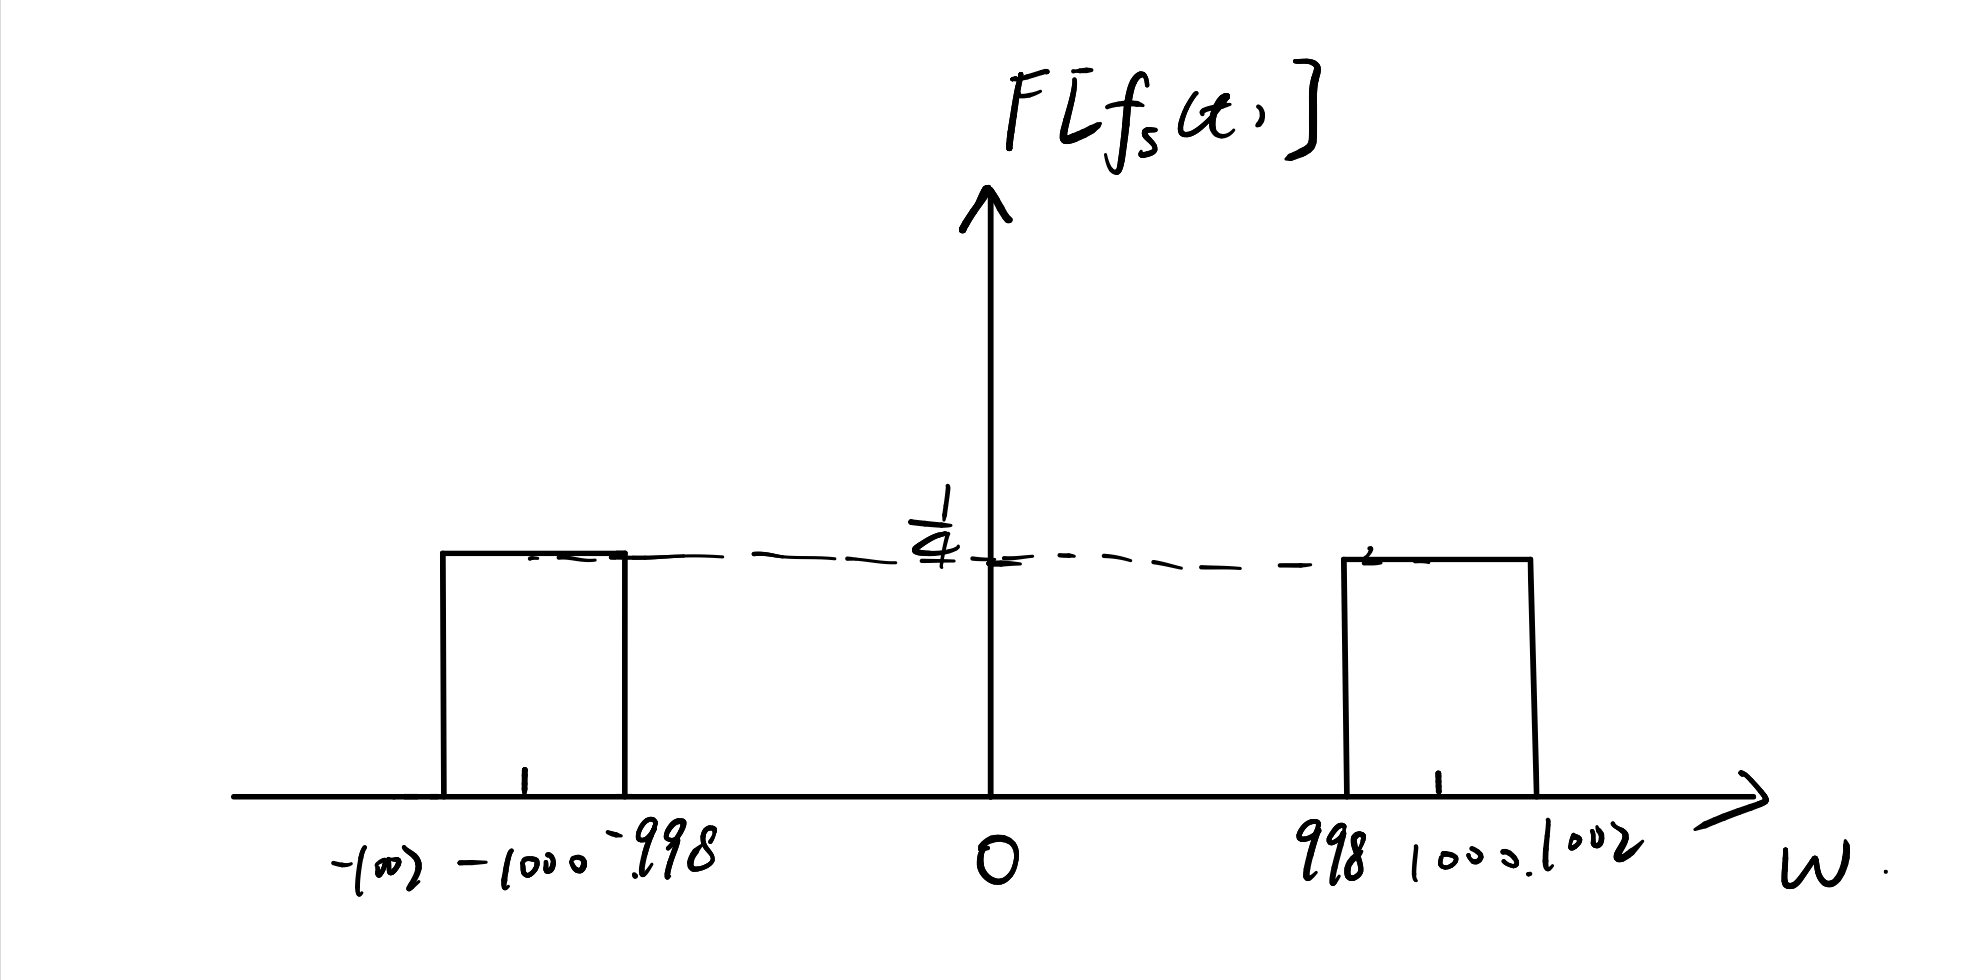
\includegraphics[width=14cm,height=8cm]{pics/p1.png}
	\caption{第一题幅度谱和相位谱}
\end{figure}
\question 已知信号
\begin{equation}
	\nonumber
	x(t) = 
	\begin{cases}
		1 + \cos(t), \qquad |t| \leq \pi \\
		0, \qquad |t| > \pi
	\end{cases}	
\end{equation}
求该信号的傅里叶变换。

\begin{solution}
	\begin{align*}
	X(jw)&=\int_{-\infty}^{\infty}x(t)e^{-jwt}dt\\
	&=\int_{-\pi}^{\pi}(1+cos(t))e^{-jwt}dt\\
	&=\int_{-\pi}^{\pi}(coswt-jsinwt)dt+\int_{-\pi}^{\pi}cost(coswt-jsinwt)dt\\	
	\end{align*}
第一项中由于$sinwt$为奇函数,故只需要计算$coswt$在$(-\pi,\pi)$上的积分,结果为$2\frac{sin\pi w}{w}$\\
接下来计算第二项$\int_{-\pi}^{\pi}cost(coswt-jsinwt)dt$,其中含$sinwt$项为奇函数,在对称区间上积分为0,故计算$\int_{-\pi}^{\pi}costcoswtdt$即可\\
\begin{align*}
	\int_{-\pi}^{\pi}costcoswtdt&=\int_{-\pi}^{\pi}\frac{1}{2}[cos(t+wt)+cos(t-wt)]dt\\
	&=\frac{1}{2}\int_{-\pi}^{\pi}cos((1+w)t)dt+\frac{1}{2}\int_{-\pi}^{\pi}cos((1-w)t)dt\\
	&=\frac{sin((1+w)\pi)}{1+w}+\frac{sin((1-w)\pi}{1-w}
\end{align*}
将两项加起来即可得到:\\
$$X(jw)=2\frac{sin\pi w}{w}+\frac{sin((1+w)\pi)}{1+w}+\frac{sin((1-w)\pi}{1-w}$$
$$=2\pi Sa(w\pi)+\pi Sa((1-w)\pi)+\pi Sa((1+w)\pi)$$

\end{solution}

\newpage
\question 已知$x_1(t)$和$x(t)$的波形图如图所示,$x_1(t)$的傅里叶变换为$X_1(j\omega)=2T \cdot Sa(\omega T)$,试利用傅里叶变换的尺度变换、位移和线性性质求$x(t)$的傅里叶变换。



\begin{solution}
	$x(t)=x_1(2t-T)-x_1(2t+T)$,故$$X(jw)=\mathcal{F}[(x_1(2t-T))]-\mathcal{F}[(x_1(2t+T))]$$
	分别求这两项\\
	\begin{align*}
		\mathcal{F}[(x_1(2t-T))]&=\mathcal{F}[(x_1(2(t-0.5T))]\\
		&=\frac{1}{2}X_1(\frac{jw}{2})e^{-\frac{jwT}{2}}
	\end{align*}
	\begin{align*}
		\mathcal{F}[(x_1(2t+T))]&=\mathcal{F}[(x_1(2(t+0.5T))]\\
		&=\frac{1}{2}X_1(\frac{jw}{2})e^{\frac{jwT}{2}}
	\end{align*}
	故\\
	\begin{align*}
		X(jw)&=\frac{1}{2}X_1(\frac{jw}{2})e^{-\frac{jwT}{2}}-\frac{1}{2}X_1(\frac{jw}{2})e^{\frac{jwT}{2}}\\
		&=TSa(\frac{wT}{2})(e^{-\frac{jwT}{2}}-e^{\frac{jwT}{2}})
	\end{align*}
\end{solution}

\newpage
\question 求图所示对称周期矩形信号的傅里叶级数,三角形式和指数形式。



\begin{solution}
	\begin{enumerate}
		\item 三角形式:
		\begin{align*}
			&a_0=\frac{1}{T}\int_{-0.5T}^{0.5T}x(t)dt=0\\
			&a_n=\frac{2}{T}\int_{-0.5T}^{0.5T}x(t)cos(nwt)dt=0\\
			&b_n=\frac{2}{T}\int_{-0.5T}^{0.5T}x(t)sin(nwt)dt=\frac{2E}{Tnw}-\frac{2E}{Tnw}cos(0.5nwT)
		\end{align*}
		将$T=\frac{2\pi}{w}$代入,得到$b_n=\frac{E}{n\pi}-\frac{E}{n\pi}cos(n\pi)$\\
		故三角形式的傅里叶级数为$x(t)=\sum\limits_{n=1}^{\infty}(\frac{E}{n\pi}-\frac{E}{n\pi}cos(n\pi))sin(nwt)$
		\item 指数形式:
			$$X_n=\frac{1}{2}a_n-\frac{j}{2}b_n=\frac{j}{2}(\frac{E}{n\pi}cos(nw)-\frac{E}{n\pi})$$
			注意到$n=0$时分母变成0,故$X_0=\frac{1}{T}\int_{-0.5T}^{0.5T}x(t)dt=0$\\
			故指数形式的傅里叶级数为$$x(t)=\sum\limits_{n=-\infty\mbox{且}n\not=0}^{\infty}\frac{j}{2}(\frac{E}{n\pi}cos(nw)-\frac{E}{n\pi})e^{jnwt}$$

	\end{enumerate}
\end{solution}
\newpage
\question 求图所示周期锯齿信号的指数形式傅里叶级数,并大致画出频谱图。


\begin{solution}
	\begin{align*}
		X_n&=\frac{1}{T}\int_0^Tx(t)e^{-jnwt}dt\\
		&=\frac{1}{T}\int_0^T(-\frac{E}{T}t+E)e^{-jnwt}dt\\
		&=-\frac{E}{T^2}\int_0^Tte^{-jnwt}dt+\frac{E}{T}\int_0^Te^{-jnwt}dt\\
		&=-\frac{E}{T^2}(-\frac{T}{jnw}e^{-jnwT})
	\end{align*}
	代入$wT=2\pi$得到$X_n=\frac{E}{j2n\pi}e^{-j\cdot 2n\pi}=\frac{E}{j2n\pi}$\\
	注意到$n=0$时分母为0,故$X_0=\frac{1}{T}\int_0^Tx(t)dt=\frac{E}{2}$\\
	所以指数形式傅里叶级数为$$x(t)=\frac{E}{2}+\sum\limits_{n=-\infty\mbox{且}n\not=0}^\infty\frac{E}{j2n\pi}e^{jnwt}$$
	频谱图如下:
\end{solution}
\begin{figure}[h]
	\centering
	\includegraphics[width=13cm,height=7cm]{pics/p5.png}
	\caption{第五题频谱图}
\end{figure}
\newpage
\question 求图所示锯齿脉冲与单周正弦脉冲的傅里叶变换。


\begin{solution}
	(a)\begin{align*}
		X(jw)&=\int_{-0.5T}^{0.5T}x(t)e^{-jwt}dt\\
		&=\int_{-0.5T}^{0.5T}\frac{2E}{T}te^{-jwt}dt\\
		&=\frac{2E}{T}\cdot(-\frac{1}{jw})(te^{-jwt}-\frac{sinwt}{w}+j\frac{coswt}{w})|_{t_1=-0.5T}^{t_2=0.5T}\\
		&=\frac{4Esin0.5wT}{Tjw^2}-\frac{2Ecos0.5wT}{jw}\\
		&=-\frac{2E}{jw}cos0.5wT+\frac{2E}{jw}Sa(0.5wT)
	\end{align*}
	注意$w=w_0$时分母为0,此时$X(jw)=X(0)=0$
	\\
	(b)\begin{align*}
		X(jw)&=\int_0^Tx(t)e^{-jwt}dt\\
		&=\int_0^T(-\frac{E}{T}t+E)e^{-jwt}dt\\
		&=-\frac{E}{T}\int_0^Tte^{-jwt}dt+E\int_0^Te^{-jwt}dt\\
		&=-\frac{E}{T}\cdot(-\frac{1}{jw})(te^{-jwt}-\frac{sinwt}{w}+j\frac{coswt}{w})|_{t_1=0}^{t_2=T}+E(\frac{sinwt+jcoswt}{w})|_{t_1=0}^{t_2=T}\\
		&=\frac{E}{Tw^2}e^{jwT}-\frac{E}{Tw^2}-\frac{Ej}{w}
	\end{align*}
	注意$w=0$时分母为0,此时$X(jw)=X(0)=\frac{ET}{2}$
	\\
	(c)记$w_0=\frac{2\pi}{T}$\\
	\begin{align*}
		X(jw)&=\int_0^Tx(t)e^{-jwt}dt\\
		&=\int_0^TEsin(w_0t)e^{-jwt}dt\\
		&=E\frac{-\frac{1}{w_0}e^{-jwt}cos(w_0t)-\frac{jw}{w_0^2}e^{-jwt}sin(w_0t)}{1-\frac{w^2}{w^2_0}}|_{t_1=0}^{t_2=T}\\
		&=\frac{w_0E}{w_0^2-w^2}(1-e^{-jwt})
	\end{align*}
	注意$w=w_0$时分母为0,此时$X(jw)=X(jw_0)=\frac{ET}{2j}$
	\\
	(d)记$w_0=\frac{2\pi}{T}$\\
	\begin{align*}
		X(jw)&=\int_{-0.5T}^{0.5T}x(t)e^{-jwt}dt\\
		&=\int_{-0.5T}^{0.5T}Esin(w_0t)e^{-jwt}dt\\
		&=E\frac{-\frac{1}{w_0}e^{-jwt}cos(w_0t)-\frac{jw}{w_0^2}e^{-jwt}sin(w_0t)}{1-\frac{w^2}{w^2_0}}|_{t_1=-0.5T}^{t_2=0.5T}\\
		&=\frac{w_0E}{w_0^2-w^2}(e^{-0.5jwT}-e^{0.5jwT})\\
		&=\frac{2jw_0E}{w^2-w_0^2}sin(0.5wT)
	\end{align*}
	注意$w=w_0$时分母为0,此时$X(jw)=X(jw_0)=\frac{ET}{2j}$
\end{solution}

\newpage
\question 分别求图所示$X(j\omega)$的傅里叶逆变换。


\begin{solution}
	(a)$X(jw)=|X(jw)|e^{j\phi(w)}=Ae^{jwt_0}$\\
	\begin{align*}
		x(t)&=\mathcal{F}^{-1}[X(jw)]=\frac{1}{2\pi}\int_{-w_0}^{w_0}X(jw)e^{jwt}dw\\
		&=\frac{A}{\pi}\cdot\frac{sinw_0t}{t_0+t}\\
		&=\frac{Aw_0}{\pi}Sa(w_0(t+t_0))
	\end{align*}
	(b)$X(jw)=|X(jw)|e^{j\phi(w)}=Ae^{j\frac{\pi}{2}sgn(w)}$\\
	\begin{align*}
		x(t)&=\mathcal{F}^{-1}[X(jw)]\frac{1}{2\pi}\int_{-w_0}^{w_0}X(jw)e^{jwt}dw\\
		&=\frac{A}{2\pi}\int_{-w_0}^{w_0}e^{j\frac{\pi}{2}sgn(w)}e^{jwt}dw\\
		&=\frac{A}{2\pi}(\int_{-w_0}^0e^{-j\frac{\pi}{2}}e^{jwt}dw+\int_0^{w_0}e^{j\frac{\pi}{2}}e^{jwt}dw)
	\end{align*}
	注意到$e^{j\frac{\pi}{2}}=cos(\frac{\pi}{2})+jsin(\frac{\pi}{2})=j,e^{-j\frac{\pi}{2}}=-j$\\
	故\begin{align*}
		x(t)&=\frac{A}{2\pi}(-j\int_{-w_0}^0e^{jwt}dw+j\int_0^{w_0}e^{jwt}dw)\\
		&=\frac{jA}{2\pi}(\frac{j-sinw_0t-jcosw_0t}{t}+\frac{sinw_0t-jcosw_0t+j}{t})\\
		&=\frac{jA}{\pi}(\frac{j-jcosw_0t}{t})\\
		&=\frac{A}{\pi t}(cosw_0t-1)
	\end{align*}
\end{solution}

\newpage
\question 利用微分定理求图所示梯形脉冲的傅里叶变换,并大致画出$\tau=2\tau_1$情况下该脉冲的频谱图。

\begin{figure}[h]
	\centering
	\includegraphics[width=\linewidth]{pics/p8-1.png}
	\caption{求导图像}
\end{figure}
\begin{solution}
	对$x(t)$分别求一、二阶导数,图像如上\\
	由微分定理,$$\mathcal{F}[\frac{d^2x(t)}{dt^2}]=(jw)^2X(jw)=-w^2X(jw)$$
	由于$\mathcal{F}[\delta(t)]=1$,
	故$$\mathcal{F}[\frac{d^2x(t)}{dt^2}]=\frac{2E}{\tau-\tau_1}e^{\frac{jw\tau}{2}}+\frac{2E}{\tau-\tau_1}e^{-\frac
	{jw\tau}{2}}-\frac{2E}{\tau-\tau_1}e^{\frac{jw\tau_1}{2}}-\frac{2E}{\tau-\tau_1}e^{-\frac{jw\tau_1}{2}}$$
	化简得\begin{align*}
		X(jw)&=-\frac{1}{w^2}\cdot\frac{2E}{\tau-\tau_1}(e^{\frac{jw\tau}{2}}+e^{-\frac{jw\tau}{2}}-e^{\frac{jw\tau_1}{2}}-e^{-\frac{jw\tau_1}{2}})\\
		&=-\frac{1}{w^2}\cdot\frac{4E}{\tau-\tau_1}(cos\frac{w\tau}{2}-cos\frac{w\tau_1}{2})\\
		&=\frac{1}{w^2}\cdot\frac{8E}{\tau-\tau_1}sin(\frac{w(\tau+\tau_1)}{4})sin(\frac{w(\tau-\tau_1)}{4})\\
		&=\frac{E(\tau+\tau_1)}{2}Sa(\frac{w(\tau+\tau_1)}{4})Sa(\frac{w(\tau-\tau_1)}{4})
	\end{align*}
	$\tau=2\tau_1$时,$X(jw)=\frac{3E\tau_1}{2}Sa(\frac{3w\tau_1}{4})Sa(\frac{w\tau_1}{4})$\\
	频谱图如下:
\end{solution}

\begin{figure}[h]
	\centering
	\includegraphics[width=\linewidth]{pics/p8-2.png}
	\caption{第八题频谱图}
\end{figure}
\newpage
\question 若已知$\mathcal{F}[x(t)] = X(j\omega)$,利用傅里叶变换的性质确定下列信号的傅里叶变换。
\begin{enumerate}[(1)]
	\item $tx(2t)$
	\item $(t-2)x(t)$
	\item $(t-2)x(-2t)$
	\item $t\frac{dx(t)}{dt}$
	\item $x(1-t)$
	\item $(1-t)x(1-t)$
	\item $x(2t-5)$
\end{enumerate}


\begin{solution}
	(1)、记$x_1(t)=x(2t),X_1(jw)=\mathcal{F}[x_1(t)]$\\
	由尺度变换特性,$X_1(jw)=\frac{1}{2}X(\frac{jw}{2})$\\
	再由频域微分特性,$\mathcal{F}[tx_1(t)]=j\cdot\frac{dX_1(jw)}{dw}$\\
	化简可得$\mathcal{F}[tx(2t)]=\frac{1}{2}\cdot j\cdot\frac{dX(\frac{jw}{2})}{dw}$\\

	(2)、由线性性,$\mathcal{F}[(t-2)x(t)]=\mathcal{F}[tx(t)]-2\mathcal{F}[x(t)]$\\
	由频域微分特性,$\mathcal{F}[tx(t)]=j\frac{dX(jw)}{dw}$\\
	化简可得$\mathcal{F}[(t-2)x(t)]=j\frac{dX(jw)}{dw}-2X(jw)$

	(3)、由线性性,$\mathcal{F}[(t-2)x(-2t)]=\mathcal{F}[tx(-2t)]-2\mathcal{F}[x(-2t)]$\\
	化简得$\mathcal{F}[(t-2)x(-2t)]=\frac{1}{2}\cdot j\cdot\frac{dX(-\frac{jw}{2})}{w}-X(-\frac{jw}{2})$\\
	
	(4)、由时域微分特性$\mathcal{F}[\frac{dx(t)}{dt}]=jw\cdot X(jw)$\\
	记$x'(t)=\frac{dx(t)}{dt},X_1(jw)=\mathcal{F}[x'(t)]=jw\cdot X(jw)$\\
	故$\mathcal{F}[tx'(t)]=j\cdot\frac{dX_1(jw)}{dw}$\\
	化简得到$\mathcal{F}[t\frac{dx(t)}{dt}]=-X(jw)-w\frac{dX(jw)}{dw}$\\

	(5)、先沿$x(t)$轴翻转,再平移,故$\mathcal{F}[x(1-t)]=X(-jw)e^{-jw}$\\

	(6)、令$x_1(t)=x(1-t)$,所求变换为$\mathcal{F}[x_1(t)]-\mathcal{F}[tx_1(t)]$\\
	先求$X_1(jw)=\mathcal{F}[x_1(t)]=X(-jw)e^{-jw}$\\
	故$\mathcal{F}[tx_1(t)]=j\cdot\frac{dX_1(jw)}{dw}$\\
	化简整理得$\mathcal{F}[(1-t)x(1-t)]=-j\cdot e^{-jw}\cdot\frac{dX(-jw)}{dw}$


	(7)、先平移五个单位,再做压缩变换,故$\mathcal{F}[x(2t-5)]=\frac{1}{2}X(j\frac{w}{2})e^{-\frac{5jw}{2}}$
\end{solution}
\newpage
\Huge{编程题报告}\\
\Large{Problem 1}\\
1.1\ 当$\tau$趋向于0时,信号变为幅度为A,周期为$T_0$的冲激信号\\
1.2\ 先计算傅里叶级数\\
\begin{align*}
	X_n&=\frac{1}{T_0}\int_{-0.5T_0}^{0.5T_0}x(t)e^{-jnwt}dt\\
	&=\frac{1}{T_0}\int_{-0.5\tau}^{0.5\tau}Ae^{-jnwt}dt\\
	&=\frac{A\tau}{T_0}Sa(0.5nw\tau)
\end{align*}\\
故$x(t)=\sum\limits_{n=-\infty}^{\infty}X_ne^{jnwt}=\frac{A\tau}{T_0}Sa(0.5nw\tau)$\\
两边同时作傅里叶变换得到$$X(jw)=\sum\limits_{n=-\infty}^{\infty}X_n\cdot2\pi\delta(w-n\frac{2\pi}{T_0})=\sum\limits_{n=-\infty}^{\infty}\frac{A\tau}{T_0}Sa(0.5nw\tau)\cdot2\pi\delta(w-n\frac{2\pi}{T_0})$$
1.3 取$A=1,T_0=1ms,\tau=\frac{T_0}{10}=0.1ms$绘图结果如下:\\
\begin{figure}[h]
	\centering
	\includegraphics[width=12cm,height=8.5cm]{pics/program1.png}
	\caption{编程题一频谱图}
\end{figure}
\ \ \ 首先,我们知道冲激信号的傅里叶变换依然是冲激信号,对于$\tau\rightarrow0$的情况,在图中可见
只在零点附近振幅较大,之后快速衰减到趋近于0,可以粗略视为冲激信号,这也正好印证了1.1的回答。\\
\newpage
\Large{Problem 2}\\
2.1\ \\
(1).随着D的增大,mse不断减小。我选取D从5000到100000,以5000为间隔绘制了D与对应的MSE的图像(用折线连接),其结果也是符合描述的\\
\begin{figure}[h]
	\centering
	\includegraphics[width=16cm,height=12cm]{pics/program2_1.png}
	\caption{D-MSE图像}
\end{figure}
(2).D 对RBF kernel 的速度没有影响,因为RBF kernel 使用高斯函数
不涉及采样过程,对RFF kernel 的速度有影响,随着采样次数D 的增加,
RFF kernel 的运行时间自然会增加。\\
如下是在D=500时取$x\_dim$=100,200,300,400,500,600,700,800,900时两个$kernel\_fn$的运行时间。

\newpage
\begin{figure}[h]
	\centering
	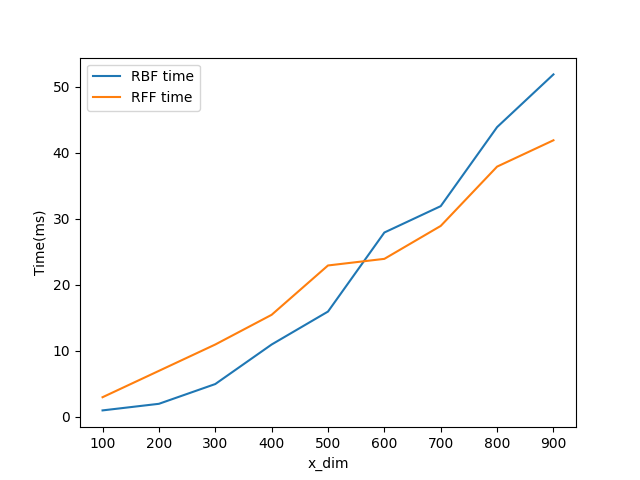
\includegraphics[width=13cm,height=8cm]{D:/Study/Grade 3/First/数字信号处理/Ass/作业-2/编程题/examples/results/Time.png}
	\caption{x dim-Time}
\end{figure}
可见,RFF确实能够提高核函数的计算速度,精度上损失也较小。
\newpage
2.2\ \\
(1).linear kernel和RBF kernel的划分结果分别如下图所示。\\
\begin{figure}[h]
	\centering
	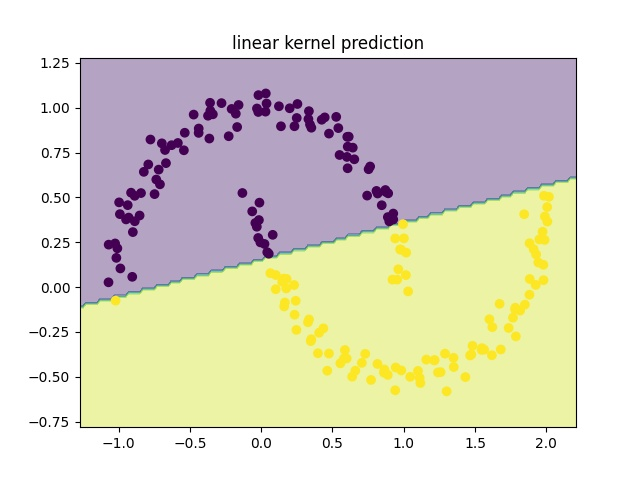
\includegraphics[width=13cm,height=8cm]{D:/Study/Grade 3/First/数字信号处理/Ass/作业-2/编程题/examples/results/linear_moon_data.jpg}
	\caption{linear kernel效果图}
\end{figure}

\begin{figure}[!h]
	\centering
	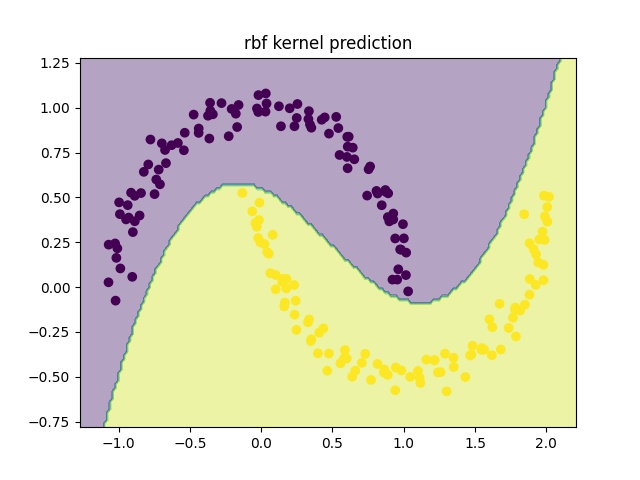
\includegraphics[width=13cm,height=8cm]{D:/Study/Grade 3/First/数字信号处理/Ass/作业-2/编程题/examples/results/rbf_moon_data.jpg}
	\caption{RBF kernel效果图}
\end{figure}
由图片可见,RBF kernel明显效果更加优异\\
\newpage
(2).下图是RFF kernel进行分类的效果图(取D=500),可见,由于RFF kernel本质上就是对
RBF kernel的近似,这二者划分出来的效果相似度很高,并且都显著优于linear kernel\\
\begin{figure}[h]
	\centering
	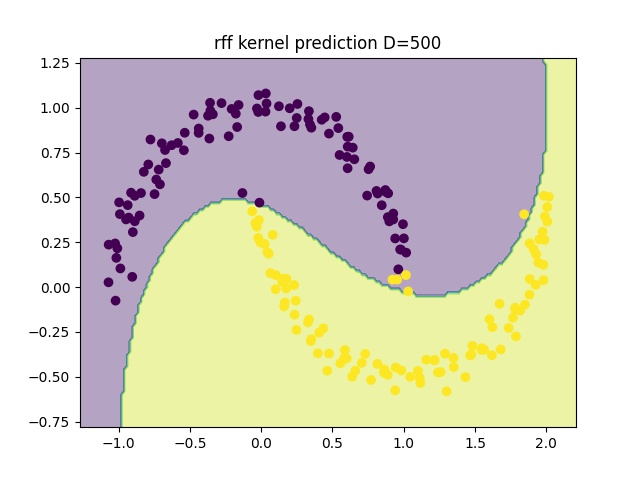
\includegraphics[width=13cm,height=7cm]{D:/Study/Grade 3/First/数字信号处理/Ass/作业-2/编程题/examples/results/rff_moon_data.jpg}
	\caption{RFF kernel效果图}
\end{figure}
(3).分别取D=500,5000,50000进行划分,得到的图片如下:\\
\begin{figure}[h]
	\centering
	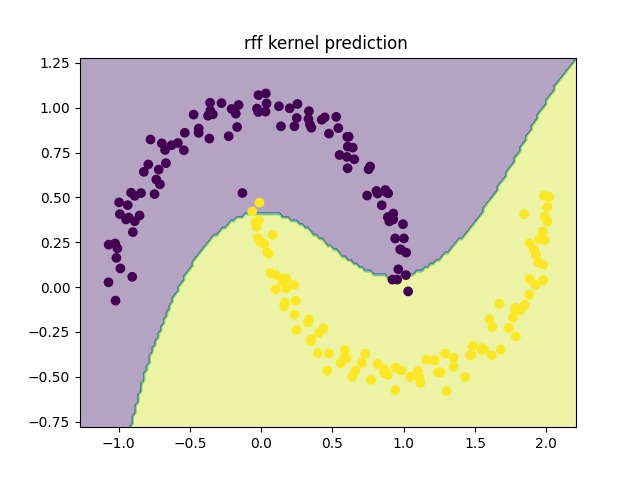
\includegraphics[width=13cm,height=7cm]{D:/Study/Grade 3/First/数字信号处理/Ass/作业-2/编程题/examples/results/rff_moon_data(D=500).jpg}
	\caption{D=500时RFF kernel效果图}
\end{figure}
\newpage
\begin{figure}[h]
	\centering
	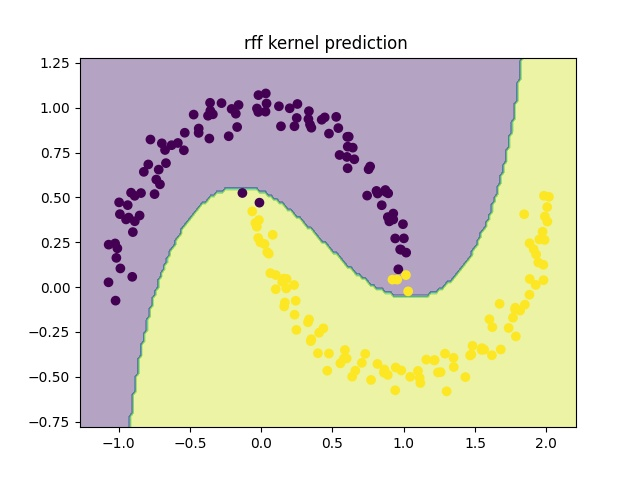
\includegraphics[width=13cm,height=7cm]{D:/Study/Grade 3/First/数字信号处理/Ass/作业-2/编程题/examples/results/rff_moon_data(D=5000).jpg}
	\caption{D=5000时RFF kernel效果图}
\end{figure}
\begin{figure}[!h]
	\centering
	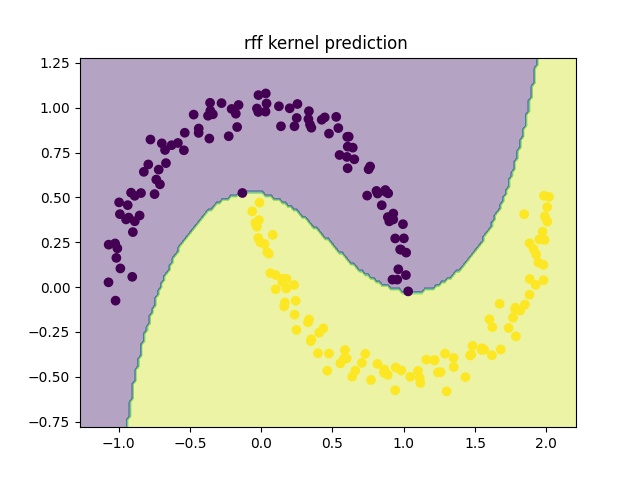
\includegraphics[width=13cm,height=7cm]{D:/Study/Grade 3/First/数字信号处理/Ass/作业-2/编程题/examples/results/rff_moon_data(D=50000).jpg}
	\caption{D=50000时RFF kernel效果图}
\end{figure}
可见,D越大,决策边界越准确。\\
当D很大时,需要花费更多的时间去做采样和矩阵乘法,自然会耗时更长\\
\newpage
2.3\ \\
(1).图像如下(D=500)\\
\begin{figure}[h]
	\centering
	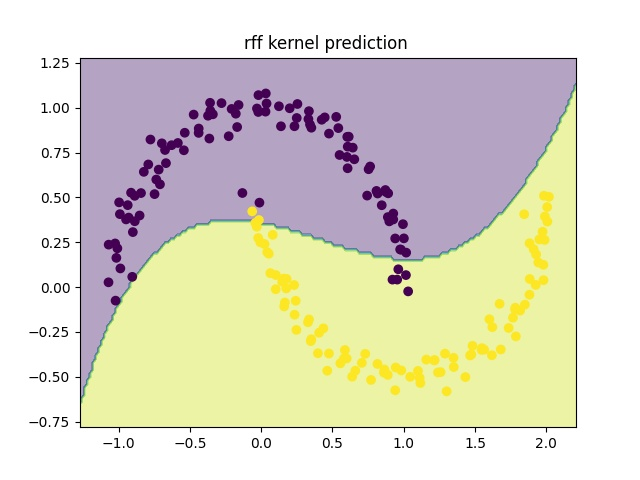
\includegraphics[width=13cm,height=7cm]{D:/Study/Grade 3/First/数字信号处理/Ass/作业-2/编程题/examples/results/rff_moon_data(修改后).jpg}
	\caption{更换linear之后的RFF}
\end{figure}
比没使用sklearn.svm.LinearSVC的时候略有提升(与Figure11相比多分对了1个样本),正确率很接近RBF了\\
(2).固定D=10000,重复了50次分类,RBF和RFF的mse图像如下:\\
\begin{figure}[h]
	\centering
	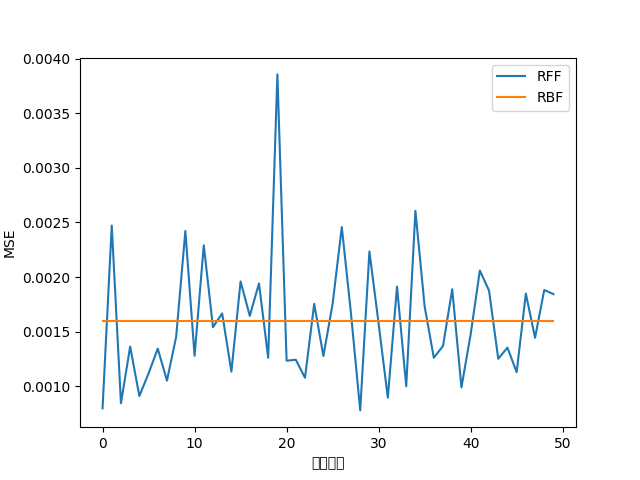
\includegraphics[width=13cm,height=7cm]{D:/Study/Grade 3/First/数字信号处理/Ass/作业-2/编程题/examples/results/p2-3.png}
	\caption{RFF,RBF的MSE对比}
\end{figure}
可见,二者性能相近,均优于线性核\\
(3).这一问中我不太明白该从何处计时算是训练、推理,因此无法给出确切的报告,不过关于速度差距的原因,我的猜测如下:\\
\ \ \ \ 样本较多时,RBF计算核矩阵的开销要大于RFF,这使得RBF的训练时间更长。\\
\ \ \ \ 至于推理用时,个人猜测可能RFF略有优势,差距并不是很明显,因为核矩阵已经计算出来了,分类过程复杂度二者相近


\end{questions}

\end{document}

